\documentclass[10pt, a4paper]{article}
\usepackage[utf8]{inputenc}
\usepackage[T1]{fontenc}
\usepackage[polish]{babel}
\usepackage[colorlinks = true,
            linkcolor = blue,
            urlcolor  = blue,
            citecolor = blue,
            anchorcolor = blue]{hyperref}
            
\usepackage{amsmath}

\usepackage{subfigure}
\usepackage{float}
\usepackage{graphicx}
\usepackage{pgfplots}
\pgfplotsset{compat=1.17}

\usepackage{biblatex}
\usepackage{csquotes}
\addbibresource{bibliografia.bib}

\title{[INZ] Notatki}
\author{Adamski Maciej}
\date{Październik 2021}

\begin{document}

\maketitle

\section{Detekcja twarzy}

\subsection{Cascading Classifier}

\subsubsection{Haar Cascade}

\subsubsection{LBP Cascade}




\subsection{Deep Neural Network}
Jeden z modułów Opencv-contrib. Służy do ładowania modeli głębokich sieci neuronowych i przepuszczeniu przez nie obrazów (lub ich części) celem wykrycia różnych obiektów.

\subsubsection{Caffemodel}
Jednym z modeli dostępnych do detekcji twarzy przy pomocy głebokich sieci neuronowych są modele Caffe (\textit{Convolutional Architecture for Fast Feature Embedding}).\\
Aktualnie używany w projekcie wzorzec caffe to \\\textit{res10{\_}300x300{\_}ssd{\_}iter{\_}140000{\_}fp16}.

\subsection{Filtrowanie wyników}
Użyte algorytmy mogą dawać w wyniku błędnie określone obszary twarzy. Z tego względu zwróconą tablicę obszarów poddaje filtrowaniu.
\begin{itemize}
    \item Pierwszym etapem jest odrzucenie obszarów, których środek znajduje się poza ustalonym pionowym obszarem (przyjałem przedział [0.25, 0.75] szerokości). Wynika to z założeń, że osoba używająca telefonu, korzysta z niego patrząc na wprost, a nie z boku. Natomiast odchył od pionu to indywidualne preferencje - dlatego nie określam poziomego obszaru.

    \begin{figure}[H]
        \begin{center}
            \subfigure[Przed filtrowaniem zależnym od położenia. Wykryte dodatkowe błędne obszary]{\label{fig:face_boundary_before}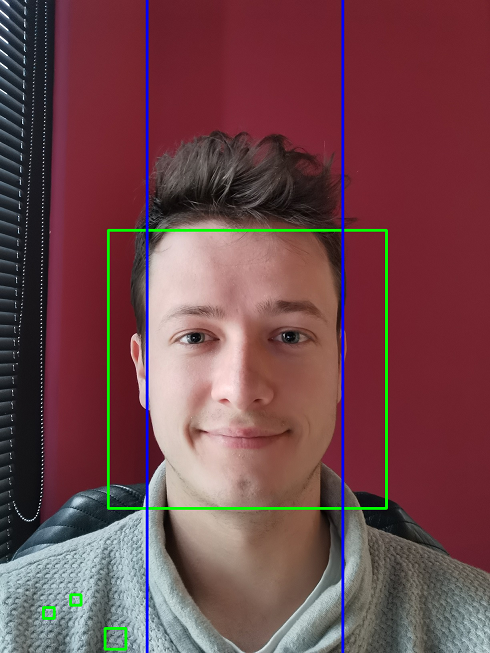
\includegraphics[scale=0.3]{images/face_filter_boundary_1.png}}
            \hspace{8mm}
            \subfigure[Po filtrowaniu. Błędne obszary odrzucone]{\label{fig:face_boundary_after}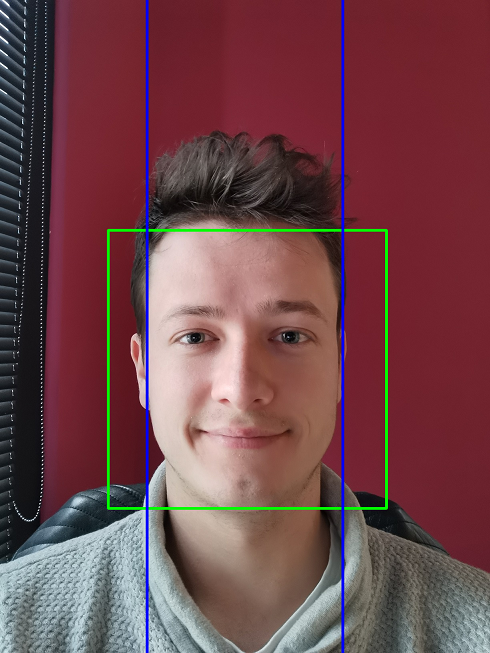
\includegraphics[scale=0.3]{images/face_filter_boundary_2.png}}
        \end{center}
        \caption{Zielone obszary - obszary, w których według klasyfikatora może znajdować się twarz. Niebieskie pasy - obszar, w którym musi znajdować się środek twarzy.}
        \label{fig:face_boundary}
    \end{figure}
    
    
    
    \item Z pozostałych obszarów wybieram ten, który zajmuje największą powierzechnię. Taki wybór motywuję tym, że twarz użytkownika telefonu na obrazie z kamery przedniej zajmuję większą część płaszczyzny, ponieważ korzystając z urządzenia nie trzymamy go bardzo daleko od siebie oraz własnymi obserwacjami zachowania algorytmów wykrywania twarzy.
    
    \begin{figure}[H]
        \begin{center}
            \subfigure[Przed filtrowaniem zależnym od wielkości. Wykryty dodatkowy błędny obszar]{\label{fig:face_size_before}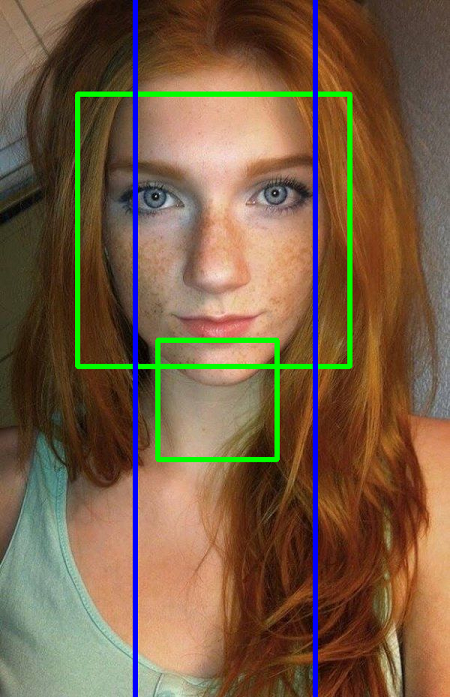
\includegraphics[scale=0.3]{images/face_filter_size_1.png}}
            \hspace{8mm}
            \subfigure[Po filtrowaniu. Błędny obszary odrzucony]{\label{fig:face_size_after}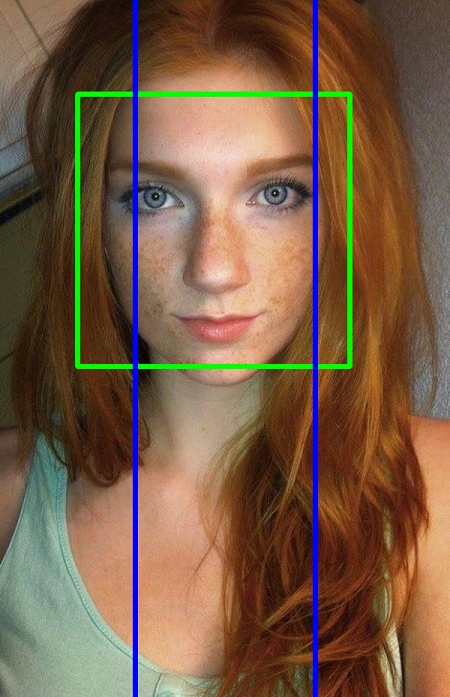
\includegraphics[scale=0.3]{images/face_filter_size_2.png}}
        \end{center}
        \caption{Kilka wykrytych obszarów w środokowej części. Wybieram najwiękzszy. \cite{readheadPortrait1}}
        \label{fig:face_size}
    \end{figure}
    
    
    
\end{itemize}


\section{Detekcja oczu}

Przed przystąpieniem do detekcji oczu należy wyznaczyć obszar, na którym wykryta została twarz. Następnie obcinając klatkę tylko do ustalonego prostokąta wykrywam oczy za pomocą Cascading Classifier - podobnie jak twarz.

Wynik który chcę uzyskać - wykryte oczy powinny się znaleźć pomiędzy naniesionymi prostkątami:

\begin{figure}[H]
    \begin{center}
        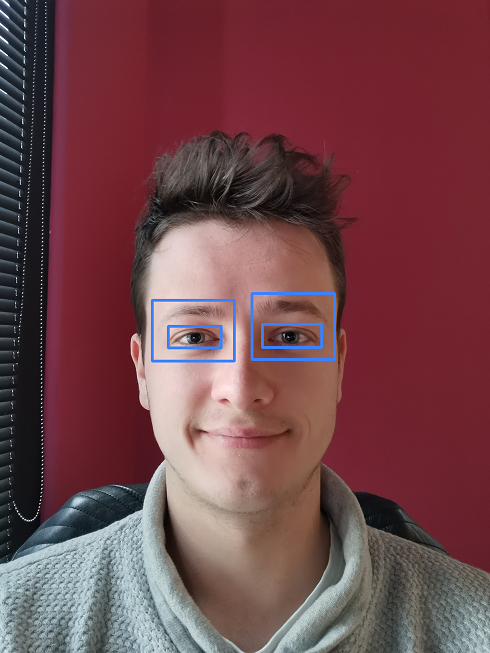
\includegraphics[scale=0.6]{images/expected_eyes_region.png}
        \caption{Przybliżony obszar oczu, który chcę wykrywać}
        \label{fig:expected_eyes_region}
    \end{center}
\end{figure}

\subsection{Obcięcie obszaru detekcji}
Dodatkowo - prócz detekcji jedynie na obszarze twarzy - zdecydowałem się zawęźić płaszczyznę przeszukiwań.
Wstępnie metodą prób i błędów dobrałem następujące parametry obcięcia obszaru:
\begin{itemize}
    \item Góra: $0.1$
    \item Dół: $0.45$
    \item Lewo: $0.1$
    \item Prawo: $0.1$
\end{itemize}

Parametr określa jaka część obszaru zostaje pominięta z poszczególnych stron.

\begin{figure}[H]
    \begin{center}
        \subfigure[Wykryty obszar twarzy]{\label{fig:eye_crop_before}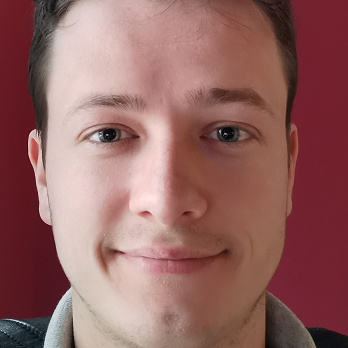
\includegraphics[scale=0.6]{images/eye_cropped_face.png}}
        \hspace{8mm}
        \subfigure[Wycięty obszar oczu]{\label{fig:eye_crop_after}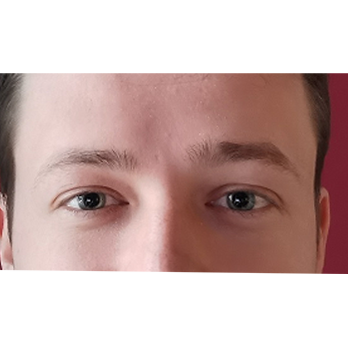
\includegraphics[scale=0.6]{images/eye_cropped_eyes.png}}
    \end{center}
    \caption{Obcięcie obszaru detekcji oczu}
    \label{fig:eye_crop}
\end{figure}

Takie zawężenie obszaru detekcji pozwoliło wyliminować cześć z błędnie oznaczonych oczu - poniżej środka twarzy czy w bok od rzeczywistego położenia:

\begin{figure}[H]
    \begin{center}
        \subfigure[Wykrywanie oczu bez dodatkowego obcięcia obszaru]{\label{fig:eye_detect_crop_before}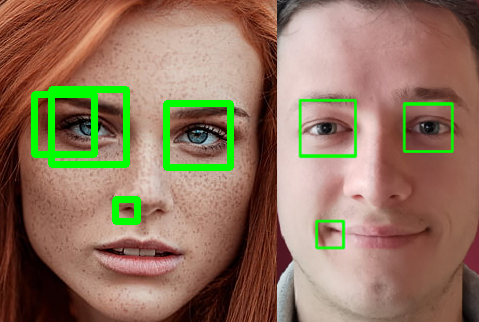
\includegraphics[scale=0.45]{images/eye_detect_before_crop_1.png}}
        \hspace{8mm}
        \subfigure[Wykrywanie oczu z dodatkowym obcięciem obszaru]{\label{fig:eye_detect_crop_after}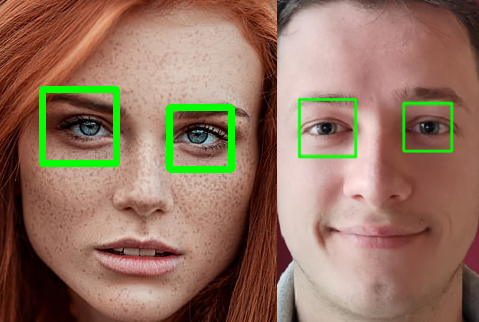
\includegraphics[scale=0.45]{images/eye_detect_after_crop_1.png}}
    \end{center}
    \caption{Poprawienie rezultatu detekcji oczu po dodatkowym obcięciu obszaru. \cite{readheadPortrait2}}
    \label{fig:eye_detect_crop}
\end{figure}

{\_\_\_\_} przyszłości zrobić testy na wielu zdjęciach wraz z wynikami przed/po w formie liczbowej. {\_\_\_\_}

\subsection{Filtrowanie wyników}

Ze względu na możliwość błędnych wskazań warto będzie wprowadzić filtrowanie wyników podobne jak w przypadku detekcji twarzy.\\
Jednym z pomysłów jest odległość między oczami 

\section{Detekcja źrenic}

Do wykrywania źrenic, najpierw musimy wyznaczyć obszar oczu. Następnie korzystając z jednych z poniższch metod ustalam interesujący nas środek. \\
Wynik, który w przybliżeniu chcę uzyskać:

\begin{figure}[H]
    \begin{center}
        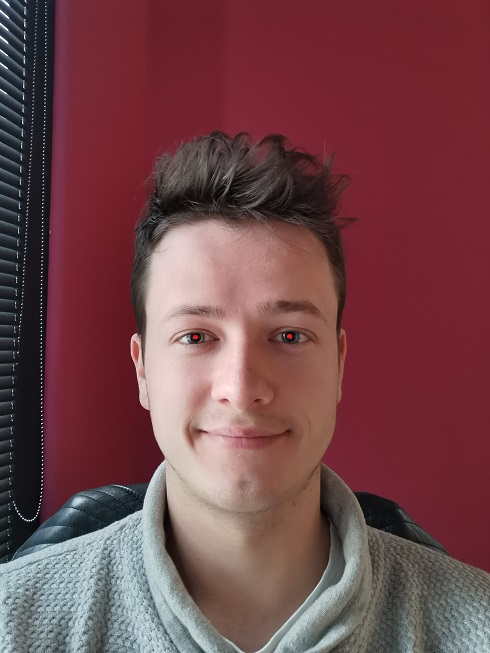
\includegraphics[scale=0.35]{images/expected_pupils.jpg}
        \caption{W przybliżeniu środek źrenic, który chcę uzyskać}
        \label{fig:expected_pupils}
    \end{center}
\end{figure}

\subsection{Algorytm CDF}
Algorytm zaimplementowany na podstawie dwóch artykułów o detekcji źrenic \cite{IMECSPupilCDFAnalysis}
\cite{EyePupilWebCam}. Opiera się w głównej mierze na progowaniu za pomocą dystrybuanty. Cały algorytm przetwarza obszar oka w skali szarości. \\
Metoda ta daje całkiem dobre i prawdopodobnie wystarczające rezultaty. \\

\begin{figure}[H]
    \begin{center}
        \subfigure[Oko skierowane w prawo]{\label{fig:pupil_cdf_left}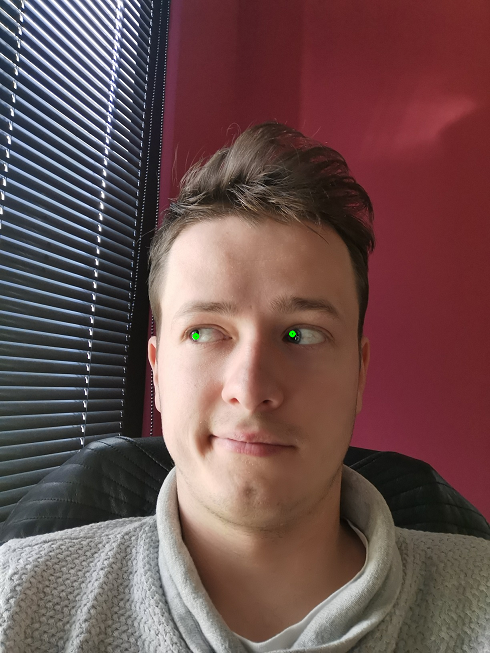
\includegraphics[scale=0.3]{images/pupil_2eyes_left_1.png}}
        \hspace{3mm}
        \subfigure[Oko skierowane na wprost]{\label{fig:pupil_cdf_center}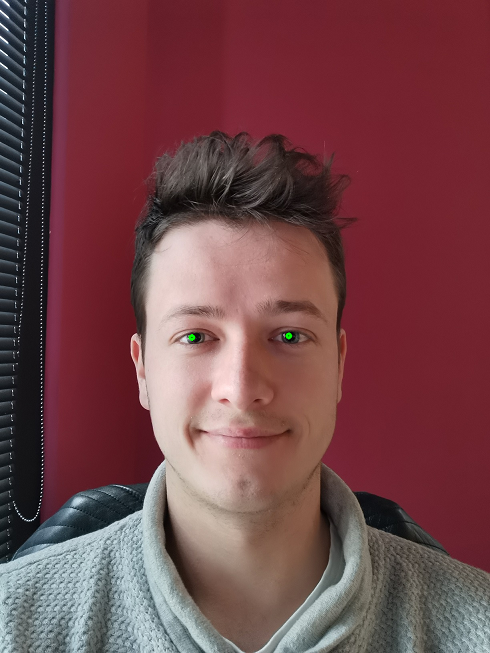
\includegraphics[scale=0.3]{images/pupil_2eyes_center_1.png}}
        \hspace{3mm}
        \subfigure[Oko skierowane w lewo]{\label{fig:pupil_cdf_right}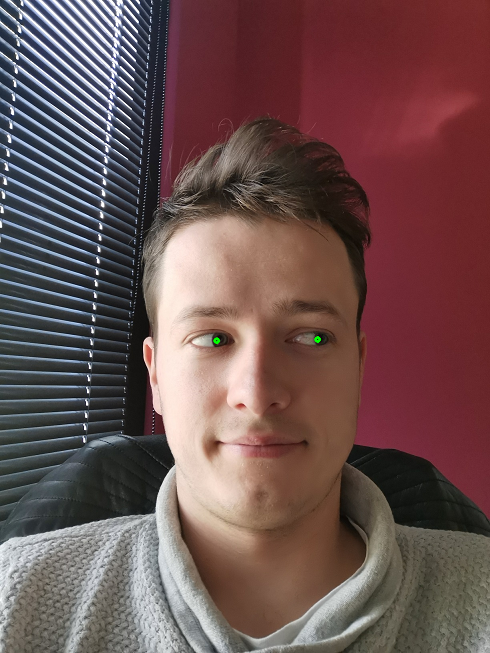
\includegraphics[scale=0.3]{images/pupil_2eyes_right_1.png}}
    \end{center}
    \caption{Rezultat wykrywania źrenic metodą CDF}
    \label{fig:cdf_results}
\end{figure}

\subsubsection{Kroki algorytmu}

\begin{itemize}
    \item Za pomocą progowania z użyciem dystrybuanty CDF tworzymy obraz binarny\\
    \begin{equation}
        CDF(r) = \sum_{w=0}^{r} p(w)
    \end{equation}
    Gdzie \textit{p(w)} to prawdopodobieństwo znalezienia punktu o jasności równej \textit{w} - określone przy pomocy dystrybuanty dystrybuanty.
    
    \begin{equation}
        I`(x, y) = 
        \begin{cases}
            255, &  CDF(I(x, y)) < \textit{a}\\
            0,   &  wpp
        \end{cases}
    \end{equation} 
    
    Gdzie \textit{I} to jasność piksela, natomiast \textit{a} to ustalony próg

    \item Na uzyskany obraz binarny nakładamy operację morfologiczną erozji (filtr minimalny), celem usunięcia pojedynczych ciemnych pikseli
    
    \item Znajdujemy najciemniejszy piksel na oryginalnym obrazie wśród tych, które mają wartość 255 (są białe) na obrazie binarnym
    
    \item Obliczamy średnią jasność pikseli w kawdracie 10x10 wokół wybranego najciemniejszego punktu
    
    \item Nakładamy erozję na obszarze 15x15 wokół wybranego punktu
    \item Na tym obszarze stosujemy progowanie
    
    \begin{equation}
        I`(x, y) = 
        \begin{cases}
            255, &  I(x, y) < AVG_I\\
            0,   &  wpp
        \end{cases}
    \end{equation}
    
    Gdzie \textit{AVG$_I$} to średnia jasność obszaru obliczona wcześniej
    
    \item Środkiem źrenicy będzie środek ciężkości białych punktów na binarnym obszarze, który uzyskaliśmy

\end{itemize}


\begin{figure}[H]
    \begin{center}
        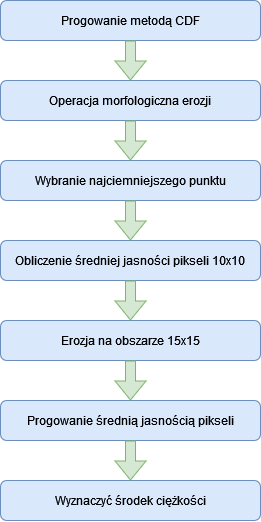
\includegraphics[scale=0.35]{images/CDF_Diagram.png}
        \caption{Kroki algorytmu metodą CDF}
        \label{fig:cdf_diagram}
    \end{center}
\end{figure}

\subsubsection{Wynik kolejnych etapów algorytmu}


\begin{figure}[H]
    \begin{center}
        \subfigure[Obszar oka w RGB]{\label{fig:cdf_rgb}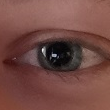
\includegraphics[scale=0.50]{images/CDF_steps/CDF_rgb_eye.png}}
        \hspace{8mm}
        \subfigure[Obszar oka w skali szarości]{\label{fig:cdf_gray}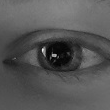
\includegraphics[scale=0.50]{images/CDF_steps/CDF_gray_eye.png}}
        \hspace{8mm}
        \subfigure[Wynik progowania CDF]{\label{fig:cdf_binary}
\includegraphics[scale=0.50]{images/CDF_steps/CDF_binary_eye_after_CDF.png}}
        
        \hfill
        
        \subfigure[Wynik erozji]{\label{fig:cdf_erode}
\includegraphics[scale=0.50]{images/CDF_steps/CDF_binary_eye_after_erode.png}}
        \hspace{8mm}
        \subfigure[Najciemniejszy punkt]{\label{fig:cdf_darkest}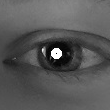
\includegraphics[scale=0.50]{images/CDF_steps/CDF_darkest_pixel.png}}
        \hspace{8mm}
        \subfigure[Obszar 15x15 wokół najciemniejszego punktu ]{\label{fig:cdf_pmi}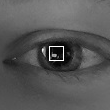
\includegraphics[scale=0.50]{images/CDF_steps/CDF_pmi.png}}
        
        \hfill
        
        \subfigure[Wynik erozji]{\label{fig:cdf_eroded_pmi}
\includegraphics[scale=0.50]{images/CDF_steps/CDF_eroded_pmi.png}}
        \hspace{8mm}
        \subfigure[Progowanie średnią jasnością pikseli]{\label{fig:cdf_threshold}
\includegraphics[scale=0.50]{images/CDF_steps/CDF_threshold_pmi.png}}
        \hspace{8mm}
        \subfigure[Wykryte położenie źrenicy]{\label{fig:cdf_pupil_detected}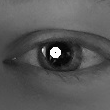
\includegraphics[scale=0.50]{images/CDF_steps/CDF_pupil_detected.png}}
        
    \end{center}
    \caption{Kolejne etapy wykrywania źrenic metodą CDF}
    \label{fig:cdf_steps}
\end{figure}

\subsection{Algorytm PF}
{\_\_\_\_} W przyszłości do testów zaimplementować algorytm PF\cite{EyePupilWebCam} {\_\_\_\_}

\subsection{Algorytm EA}
{\_\_\_\_} W przyszłości do testów zaimplementować algorytm EA\cite{EyePupilWebCam} {\_\_\_\_}

\section{Landmarks}

Są to punkty nakładane na twarz wokół interesujących obszarów - takich jak oczy, nos czy usta. Pozwalają określić położenie, rozmiar czy kształt tych obiektów. Mogą być również użyte do predykcji czy mamy zamknięte/otwarte oczy lub czy się uśmiechamy. 

\subsection{OpenCV-contrib}
Dodatkowe moduł opencv facemark (\textit{OpenCV-contrib}) zawiera trzy algorytmy detekcji landmarków:

\begin{itemize}
    \item Kazemi
    \item AAM
    \item LBF
\end{itemize}

\subsubsection{FacemarkLBF}

Używając metody FacemarkLBF oraz modelu \textit{lbfmodel.yaml} określiłem punkty orientacyjne twarzy. \cite{landmarkSatyaMallick}

\begin{figure}[H]
    \begin{center}
        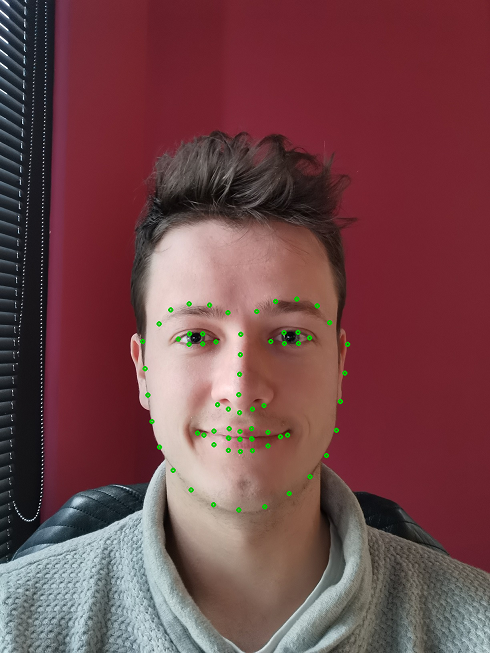
\includegraphics[scale=0.6]{images/landmarks_1.png}
        \caption{Twarz z naniesionymi landmarkami}
        \label{fig:landmarks_1}
    \end{center}
\end{figure}

\section{EAR - Eye Aspect Ratio}
Metoda wykorzystująca landmarki na twarzy. Posiadając oznaczone za pomocą tej metody oczy możemy obliczyć tzw. \textit{EAR}, czyli stosunek otwarcia oczu - wysokość do szerokości widocznej części gałki ocznej. \cite{EARRaspberryPi} \cite{eyeBlinkEARRosebrock}\\

Zależnie od ilości punktów wokół oka będzie różny wzór obliczania EAR.\\
Dla 6 punktów:
\begin{equation}
    EAR = \frac{dist(L_0, L_1) + dist(L_2, L4)}{2 * dist(L_3, L_5)}
\end{equation}
\\
Natomiast, dla 4 punktów:
\begin{equation}
    EAR = \frac{dist(L_0, L_2)}{dist(L_1, L_3)}
\end{equation}

Gdzie \textit{$L_x$} to kolejne landmarki dokoła oczu, a \textit{dist} to odległość między dwoma punktami (odległość euklidesowa).\\

W teorii otwarte oczy będą miały większy wymiar liczbowy EAR, niż oczy zamknięte. Na zdjęciu poniżej widać, że oko otwarte ma większe odległości między punktami pionowymi niż w przypadku  oka zamkniętego. 

\begin{figure}[H]
    \begin{center}
        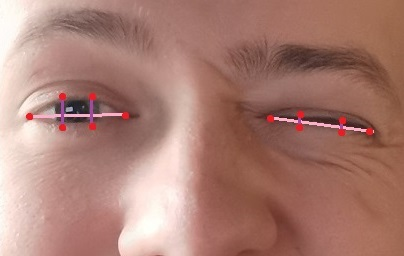
\includegraphics[scale=0.35]{images/theoretical_eye_landmarks.jpg}
        \caption{Teoretyczny rozmieszczene landmarków wokół oczu wraz z naniesionymi połączeniami do obliczenia EAR}
        \label{fig:theoretical_eye_landmarks}
    \end{center}
\end{figure}


\subsection{Testowanie z użyciem landmarków LBF opencv-contrib
}

\subsubsection{Test z użyciem kamery na żywo}

Wykonałem kilka krótkich testów z użyciem obrazu pochodzącego z przedniej kamery telefonu. 
\\
Poniżej znajdują się trzy testy, na których mrugnąłem tylko raz - lewym okiem, prawym i oboma na raz.

\begin{figure}[H]
    \centering
    \begin{tikzpicture}
        \begin{axis}[
            xlabel = {Nr klatki obrazu z kamery},
            ylabel = {EAR},
            height = 0.5\linewidth,
            width = \linewidth,
            ymin= {0.10},
            ymax={0.30},
            ytick = {0.10, 0.12, 0.14, 0.16, 0.18, 0.20, 0.22, 0.24, 0.26, 0.28, 0.30},
            ymajorgrids = {true},
        ]
            \addplot[color=blue, mark=square*] table [x=x, y=a, col sep=comma] {logs/ear_left_1.csv};
            \addplot[color=red, mark=square*] table [x=x, y=b, col sep=comma] {logs/ear_left_1.csv};
        \end{axis}
    \end{tikzpicture}
    \caption{Mrugnięcie lewym okiem}
    \label{fig:left_eye_blink}
\end{figure}


\begin{figure}[H]
    \centering
    \begin{tikzpicture}
        \begin{axis}[
            xlabel = {Nr klatki obrazu z kamery},
            ylabel = {EAR},
            height = 0.5\linewidth,
            width = \linewidth,
            ymin= {0.10},
            ymax={0.30},
            ytick = {0.10, 0.12, 0.14, 0.16, 0.18, 0.20, 0.22, 0.24, 0.26, 0.28, 0.30},
            ymajorgrids = {true},
        ]
            \addplot[color=blue, mark=square*] table [x=x, y=a, col sep=comma] {logs/ear_right_1.csv};
            \addplot[color=red, mark=square*] table [x=x, y=b, col sep=comma] {logs/ear_right_1.csv};
        \end{axis}
    \end{tikzpicture}
    \caption{Mrugnięcie prawym okiem}
    \label{fig:right_eye_blink}
\end{figure}

\begin{figure}[H]
    \centering
    \begin{tikzpicture}
        \begin{axis}[
            xlabel = {Nr klatki obrazu z kamery},
            ylabel = {EAR},
            height = 0.5\linewidth,
            width = \linewidth,
            ymin= {0.10},
            ymax={0.30},
            ytick = {0.10, 0.12, 0.14, 0.16, 0.18, 0.20, 0.22, 0.24, 0.26, 0.28, 0.30},
            ymajorgrids = {true},
        ]
            \addplot[color=blue, mark=square*] table [x=x, y=a, col sep=comma] {logs/ear_both_1.csv};
            \addplot[color=red, mark=square*] table [x=x, y=b, col sep=comma] {logs/ear_both_1.csv};
        \end{axis}
    \end{tikzpicture}
    \caption{Mrugnięcie oboma oczami na raz}
    \label{fig:both_eyes_blink}
\end{figure}


Testy z pojedynczym mruganiem w krótkim okresie czasu dają przyzwoite wyniki i można na nich okreslić moment mrugania. W szczególności przy mrugnięciu jednym okiem.\\

Poniżej rozciągnąłem w czasie test na sekwencje kilku mrugnięć.

\begin{figure}[H]
    \centering
    \begin{tikzpicture}
        \begin{axis}[
            xlabel = {Nr klatki obrazu z kamery},
            ylabel = {EAR},
            height = 0.5\linewidth,
            width = \linewidth,
            ymin= {0.10},
            ymax={0.30},
            ytick = {0.10, 0.12, 0.14, 0.16, 0.18, 0.20, 0.22, 0.24, 0.26, 0.28, 0.30},
            ymajorgrids = {true},
        ]
            \addplot[color=blue, mark=square*] table [x=x, y=a, col sep=comma] {logs/ear_long_1.csv};
            \addplot[color=red, mark=square*] table [x=x, y=b, col sep=comma] {logs/ear_long_1.csv};
        \end{axis}
    \end{tikzpicture}
    \caption{Kilka mrugnięć}
    \label{fig:multi_blinks_1}
\end{figure}

\begin{figure}[H]
    \centering
    \begin{tikzpicture}
        \begin{axis}[
            xlabel = {Nr klatki obrazu z kamery},
            ylabel = {EAR},
            height = 0.5\linewidth,
            width = \linewidth,
            ymin= {0.10},
            ymax={0.30},
            ytick = {0.10, 0.12, 0.14, 0.16, 0.18, 0.20, 0.22, 0.24, 0.26, 0.28, 0.30},
            ymajorgrids = {true},
        ]
            \addplot[color=blue, mark=square*] table [x=x, y=a, col sep=comma] {logs/ear_long_2.csv};
            \addplot[color=red, mark=square*] table [x=x, y=b, col sep=comma] {logs/ear_long_2.csv};
        \end{axis}
    \end{tikzpicture}
    \caption{Kilka mrugnięć}
    \label{fig:multi_blinks_2}
\end{figure}

\begin{figure}[H]
    \centering
    \begin{tikzpicture}
        \begin{axis}[
            xlabel = {Nr klatki obrazu z kamery},
            ylabel = {EAR},
            height = 0.5\linewidth,
            width = \linewidth,
            ymin= {0.10},
            ymax={0.30},
            ytick = {0.10, 0.12, 0.14, 0.16, 0.18, 0.20, 0.22, 0.24, 0.26, 0.28, 0.30},
            ymajorgrids = {true},
        ]
            \addplot[color=blue, mark=square*] table [x=x, y=a, col sep=comma] {logs/ear_long_3.csv};
            \addplot[color=red, mark=square*] table [x=x, y=b, col sep=comma] {logs/ear_long_3.csv};
        \end{axis}
    \end{tikzpicture}
    \caption{Kilka mrugnięć}
    \label{fig:multi_blinks_3}
\end{figure}

Tu również z dużym prawdopodobieństwem można okreśilć, w których klatkach wystąpiło mrugnięcie - widać gwałtowne obniżenie wartości EAR.
\\
Najlepsze wyniki były w przypadku pierwszego testu, ponieważ widać wtedy znaczną różnicę EAR między otwartym ($\sim0.26 - 0.30$), a zamkniętym okiem ($\sim0.12-0.18$). Na pozostałych testach różnice nie były już tak znaczące - na ostatnich dwóch wykresach otwarte i zamknięte oko ma niewielką różnicę w EAR. Takie małe różnice wyników mogą uniemożliwić prawidłową detekcję.

\vspace{3mm}
W każdym z przypadków testowych EAR dla jednego i drugiego oka prawie się pokrywają. Nawet przy mruganiu tylko jednym. Nie pozwoli to więc okręślić, którym okiem użytkownik mrugał.

\vspace{3mm}

Niewątpliwą trudnością w przypadku tej metody byłoby określenie progu wartości EAR, które zakwalifikowałbym jako mrugnięcie. Patrząc na wykresy powyżej można by przyjąć, że jest to wartość koło $~0.18$. Jednak w przypadku ostatecznego wyboru tej metody wymagałoby to dodatkowych badań celem określenia tej wartości.


\subsubsection{Niedokładność nakładania landmarków}

Patrząc jednak na położenie tych landmarków wokół oczu mam wątpliwości co do skuteczności tej metody:

\begin{figure}[H]
    \begin{center}
        \subfigure[]{\label{fig:landmarks_accuracy_1}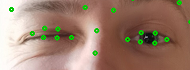
\includegraphics[scale=1.6]{images/landmarks_accuracy_1.png}}
        \hspace{8mm}
        \subfigure[]{\label{fig:landmarks_accuracy_2}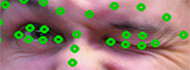
\includegraphics[scale=1.6]{images/landmarks_accuracy_2.png}}
    \end{center}
    \caption{Landmarki na oczach otwartych/zamkniętych}
    \label{fig:landmarks_accuracy_}
\end{figure}

Jak widać algorytm całkiem dobrze radzi sobie z rozmieszczeniem landmarków w przypadku otwartych oczu. Natomiast gdy oczy są zamknięte widać dużą niedokładność, która na pewno w dużym stopniu utrudnia prawidłową detekcję mrugnięcia.

\printbibliography

\end{document}
